%% LaTeX2e class for student theses
%% sections/main/3_approach.tex
%%
%% Karlsruhe University of Applied Sciences
%% Faculty of  Computer Science and Business Information Systems
%%
%% --------------------------------------------------------
%% | Derived from sdqthesis by Erik Burger burger@kit.edu |
%% --------------------------------------------------------


\chapter{Approach}
\label{ch:Approach}

This chapter describes the order and duration for processing the identified tasks, in accordance with the design specifications outlined in the previous Chapter \ref{ch:Requirements Engineering}. 
For this purpose, this work is divided into two parts, which will later serve to classify the aforementioned challenges.
The first part is theoretical, including the paper's preparation and research to understand the problem. 
The second part afterward is practical, encompassing the tasks needed to implement the system. \\
\noindent In order to aid planning, timestamps are estimated for each task or logical unit of tasks to provide reference points during the processing of corresponding dedicated work packages. 
A logical unit, as used here, refers to a coherent cluster of individual tasks that share content or functionality and can be worked on simultaneously. Working on one task without the others would be less significant.
The standard duration for processing a task or unit is set at two weeks (10 days) typically, to ensure sufficient time for completion. The duration may differ in certain cases and is determined based on the relevance and volume of related challenges. 
After describing the two conceptual parts alongside their respective tasks and processing times, this chapter concludes with a comparison of the planned procedure to the actual one.

\section{Theoretical Part}
\label{ch:Approach:sec:Theoretical Part}

With regard to the delimitation of the problem space and the synthesis of the central problem, the main aspect of the theoretical part of this work consists of a comprehensive literature review.
This involves analyzing existing work on reservation processes used for managing \acrshortpl{cs} and allocating charging infrastructure to a specific \acrshort{evu} within a limited time frame, using various methods.
With regards to the default processing time mentioned earlier, the duration for compilation as well as analysing articles and field projects related to this area is set to one month. 
The expected result should be used as the groundwork for the subsequent practical part, which is summarised in Chapter \ref{ch:Literature Review}.
As well as examining the current state of reservation systems, this review process defines a boundary for the necessary fundamentals of contextualization, resulting in Chapter \ref{ch:Fundamentals}.
Therefore, systematic requirements engineering, taking into account the facts gathered during the research phase and the collection of baselines, using a customised scenario to select relevant use cases, results in Chapter \ref{ch:Requirements Engineering}.
Chapter \ref{ch:Design} presents the design phase, which follows the summarized requirements in Chapter \ref{ch:Requirements Engineering} and the results of the literature review in Chapter \ref{ch:Literature Review}. During this phase, mockups of the relevant interfaces as well as the underlying processes will be created.
With the help of these designed concepts, the actual implementation of the reservation module resulting in Chapter \ref{ch:Implementation} takes place.
Subsequently, the theoretical section concludes by validating the achieved functionality and presenting the final results, culminating in \ref{ch:Analysis and Validation}. Potential avenues for further research are also highlighted.

\section{Practical Part}
\label{ch:Approach:sec:Practical Part}

The practical part utilizes the results of the theoretical phase, as described in Section \ref{ch:Approach:sec:Theoretical Part}. Starting with the analysis of the current state of the applications used for the development of the prototypical reservation approach of this work, the final step is the implementation of the solution, taking into account the elaborated constraints and requirements.
Seven iterations covering the implementation steps for the use cases described in Section \ref{ch:Requirements Engineering:sec:Use Cases} were conducted, commencing from the end of the theoretical phase that includes four weeks of literature research and information gathering, until the end of the processing stage.
This allows for a six--week buffer to address any unforeseen features, correct any issues with the implemented logic, and complete the documentation tasks related to the theoretical part.
Following this, a list summarising the scheduled iterations and associated timeframes will be provided.

\begin{multicols}{2}
\begin{description}
    \item[Iteration 1] 18.04.2023 -- 01.05.2023
    \item[Iteration 2] 02.05.2023 -- 15.05.2023
    \item[Iteration 3] 16.05.2023 -- 29.05.2023
    \item[Iteration 4] 30.05.2023 -- 12.06.2023
\end{description}
\begin{description}
    \item[Iteration 5] 13.06.2023 -- 26.06.2023
    \item[Iteration 6] 27.06.2023 -- 10.07.2023
    \item[Iteration 7] 11.07.2023 -- 24.07.2023
\end{description}
\end{multicols}

\noindent According to this iterative model, a functional increment of the resulting software should be provided after each iteration.

\section{Actual Course Of Action}
\label{ch:Approach:sec:Actual Course Of Action}

As there is a limited amount of available research and existing projects on reservation features for the management of \acrshortpl{cs} and charging infrastructure, the analysis and setup of the \textit{Open e--Mobility} \cite{noauthor_github_nodate,noauthor_github_nodate-1,noauthor_github_nodate-2,noauthor_github_nodate-3} solution and its particular components commenced one day earlier.
Consequently, some adjustments have been made to the above timescales for the general processing of the relevant parts.
Beginning with the identification of missing functionality required for the subsequent implementation of the customized processes.
The first step was to investigate the \textit{e--mobility charging stations simulator} \cite{noauthor_github_nodate-3} for local simulation of a customizable charging infrastructure.
Because of the identified feature gap regarding missing reservation capabilities conforming with \acrshort{ocpp} 1.6 \cite{noauthor_ocpp_nodate}, the implementation of this crucial feature for testing and evaluation purposes was included as preliminary work for the \textit{Open e--Mobility} team.
After the team members successfully reviewed the implemented logic and minor reworks of the code base, the changes were merged into the standard product.
Now, the extended \acrshort{cs} simulator was then used as a reservable charging infrastructure for the subsequent iterations.
Particularly, to validate the implementation of reservations compliant with version 1.6 of the \acrshort{ocpp} protocol, considering both pre--existing functionalities in the backend application and the adaptations according to this work.
This included not only the backend development but also the implementations within the frontend application during iterations three and four.
Due to the partially existing features mentioned above, the third iteration takes less time than expected, resulting in an earlier commencement of the relevant functions within the web frontend.
In light of the time savings achieved in the preceding iterations, the fifth iteration for implementing the custom reservation function began prematurely as well. 
To account for the unexpected scope of required operations alongside an end--to--end development approach, the author decided to merge the fifth and sixth iterations, resulting in an extended fifth iteration and a total of six iterations instead of the originally planned seven iterations.
Because of the previous schedule adjustments, the final iteration also started earlier and was completed later than intended. 
Primarily referring to the incidence of bugs and further requirements to manage reservations internally.
The resulting schedule, including the iterations, their specific duration, and the corresponding tasks, can be found in Table \ref{tab:development-iterations} below.

\begingroup
\setlength{\tabcolsep}{10pt} % Default value: 6pt
\renewcommand{\arraystretch}{1.5} % Default value: 1
\begin{table}[h]
    \centering
    \caption{Schedule for implementing the reservation feature designed in this study.}
    \begin{tabular}{c|c|c|m{7cm}}
        Iteration & From & To & Objective \\
        \hline
        1 & 17.04.2023 & 28.04.2023 & Feature gap detection within the existing application \\
        2 & 01.05.2023 & 12.05.2023 & Adjustments to the \textit{e--mobility charging stations simulator} \cite{noauthor_github_nodate-3} to support reservations complying to \acrshort{ocpp} version 1.6 \\
        3 & 15.05.2023 & 19.05.2023 & Implementation of \acrshort{ocpp} 1.6 reservation functionality in the backend application \\
        4 & 22.05.2023 & 02.06.2023 & Implementation of \acrshort{ocpp} 1.6 reservation functionality in the web frontend application \\
        5 & 05.06.2023 & 30.06.2023 & Implementation of customized reservation process in the frontend and backend applications \\
        6 & 03.07.2023 & 28.07.2023 & Implementation of \acrshort{ocpp} 1.6 reservation functionality and the customized reservation process inside the mobile application \\
    \end{tabular}
    \label{tab:development-iterations}
\end{table}
\endgroup

\noindent Besides implementing the reservation system features, this work covered other tasks related to the \textit{Green4EVer} \cite{noauthor_hka_nodate} project, although they were only indirectly connected to this work.
The decision to include these tasks is primarily based on the simplification of future deployment scenarios, such as demonstration or test cases, which require an automated and reliable setup.
Therefore, this section mentions these tasks in addition to a brief explanation of the challenge. A detailed description is omitted from both the subsequent \textit{Design} chapter \ref{ch:Design} and the \textit{Implementation} chapter \ref{ch:Implementation} according to no direct relation to the primary problem that this work covers.

\begin{description}
    \item[Task 1 -- MongoDB Manifests] As the public repository offers no other deployment options, the only available one was containerization and operation using the Docker Compose orchestration tool \cite{noauthor_overview_2023}. 
    To offer a more scalable and robust solution, the industry standard for deploying containerized applications, therefore, recommends employing \acrfull{k8s} \cite{noauthor_produktionsreife_nodate} as a sophisticated orchestrator. This led to this first task. 
    Nevertheless, the manifest files essential for creating a \textit{StatefulSets} \cite{noauthor_statefulsets_nodate} deployment, a standard way for deploying database applications inside \acrshort{k8s}, were still not yet included in the current project. 
    Hence, the MongoDB \cite{noauthor_mongodb_nodate} database's custom setup, including test data and users, already existing as part of the local setup, was employed as a blueprint for creating the necessary manifests required for the deployment.
    \item[Task 2 -- MongoDB Helm Chart] To further reduce the effort required to deploy the database application to the orchestration instances, the Helm \cite{noauthor_helm_nodate} toolbox and its charts for encapsulating \acrshort{k8s} manifests are integrated.  
    From the manifest files created in \textbf{task 1}, the corresponding Helm charts for the deployment are created, providing parameterization of a namespace and all required resources, such as \textit{PersistentVolumes} \cite{noauthor_persistent_nodate}, \textit{ConfigMaps} \cite{noauthor_configmaps_nodate} or \textit{Namespaces} \cite{noauthor_namespaces_nodate}. 
    \item[Task 3 -- \acrshort{k8s} Deployment] For the integration of the remaining applications of the solution, additional Helm charts could be organized for the backend and the frontend application. 
    Regarding the limited resources provided by the used orchestration service, the new charts required further modifications to integrate with the MongoDB chart and the deployment restrictions of the project. This involves a shift from the predefined microservice--based deployment strategy to a monolithic approach resulting in reduced resource allocation.
    \item[Task 4 - Ingress Deployment \& Public Availability] In order to access the applications within the cluster, it is necessary to use an \textit{Ingress} \cite{noauthor_ingress_nodate} acting as a reverse proxy. 
    Therefore, this ingress must be located within the \textit{Namespace} the application lives in.
    Alongside the charts for the backend and frontend mentioned in \textbf{task 3}, the collection includes a configuration for deploying an NGINX ingress controller \cite{noauthor_nginx_nodate} using the predefined ingress class. 
    In combination with a public \acrshort{dn} and the corresponding \acrshort{ip} address, the final stage of the deployment consisted of configuring the ingress deployment and registering it at a \acrshort{dn} service.
\end{description}

\newpage

\noindent As a result, the \acrshort{k8s} setup shown in Figure \ref{fig:k8s-setup}, considers a deployment scenario that includes all the required components within a custom namespace, referred to in this project as \verb|ev|. 
Alongside the particular applications, the namespace includes an NGINX ingress controller with a publicly accessible \acrshort{dn}, and a MongoDB database with built--in reinitialization of custom test data and users.
In terms of application distribution, only one node is used with multiple pods within the respective cluster.

\begin{figure}[h]
    \centering
    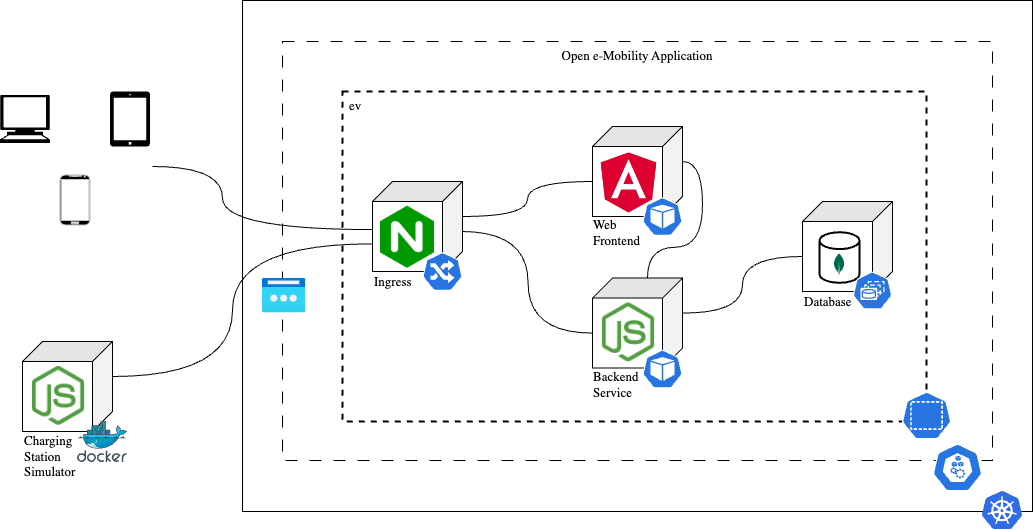
\includegraphics[scale=0.4]{resources/images/main/3_approach/KubernetesDeployment.png}
    \caption{Elaborated \acrshort{k8s} deployment architecture for the concerned solution.}
    \label{fig:k8s-setup}
\end{figure}
